The optimization model is used here as a counterfactual probe rather than as the final scientific product. For each city-event, it reveals a recovery-value field over candidate actions indexed by location, time, intervention primitive, and piecewise-linear deployment segment. The learning task is therefore not to predict a binary optimizer selection, which can be unstable under ties and near-optimal alternatives. Instead, the target is the marginal recovery value of action tokens and the lower-dimensional laws that explain where this value appears.

\subsection{Action-Level Marginal Value}

Single-action LP probes show that the correct local label is the small-signal derivative of the recovery objective, not the total finite deficit area available at a location. Across 42 representative probes, the small-signal label has Spearman correlation 0.8540 with direct LP gains and median LP-to-label ratio 1.0000, whereas the finite-area label has Spearman correlation 0.1146. This distinction matters because a location can contain large finite loss but still have low marginal value if the first unit of resource does not reach exposed future loss efficiently.

For the first deployment segment, the recovered law can be written schematically as
\begin{equation}
v_{i,t,k}^{(0)}
  \propto
  \frac{
    H_{i,t,k}^{+}
    \cdot E_{i,k}
    \cdot \eta_{i,t,k}
  }{
    c_{i,t,k} \cdot L_0
  },
\end{equation}
where \(H_{i,t,k}^{+}\) is the active future horizon over which the intervention can still reduce positive loss, \(E_{i,k}\) is the relevant OD exposure term, \(\eta_{i,t,k}/c_{i,t,k}\) is effectiveness per unit cost, and \(L_0\) is the no-intervention event loss used for normalization. For restoration and temporary capacity primitives, the exposure term is destination-side functional importance because reducing a destination deficit propagates through OD dependence. For substitution or control, the exposure term is origin weight because the primitive directly shields origin-level experienced loss.

This gives the first recoverability law:
\begin{quote}
Marginal recovery value is activated when future persistent deficit overlaps with exposed OD dependence and feasible intervention efficiency.
\end{quote}

Simple normalized action features can recover much of this value field across cities. A leave-one-city-out surrogate obtains mean Spearman correlation 0.8866 and mean top-5 percent value capture 0.7640. The symbolic activated law itself captures the top marginal-value field by construction, while exposure-only, deficit-only, and structure-only rankings are weaker and incomplete.

To test whether this structure requires a complex black-box surrogate, we train a factorized leave-one-city-out ridge action-value model with increasing feature complexity and evaluate it using within-event top-tail metrics. A deficit-only model captures 0.7297 of oracle top-5 percent value. Adding OD exposure increases this to 0.8350, while adding static structure and substitution proxies alone does not improve cross-city top-tail capture. Adding time window, feasibility, intervention type, and event context raises top-5 percent capture to 0.9624. A seven-feature low-dimensional factorized model using only delay feasibility, future horizon, OD exposure, efficiency, and intervention type already reaches 0.9375. By contrast, adding unconstrained high-dimensional interaction terms to the full model lowers top-5 percent capture from 0.9624 to 0.9511 in leave-city validation. Thus the evidence favors a compact activated structure rather than arbitrary interaction complexity.

\begin{figure}[t]
  \centering
  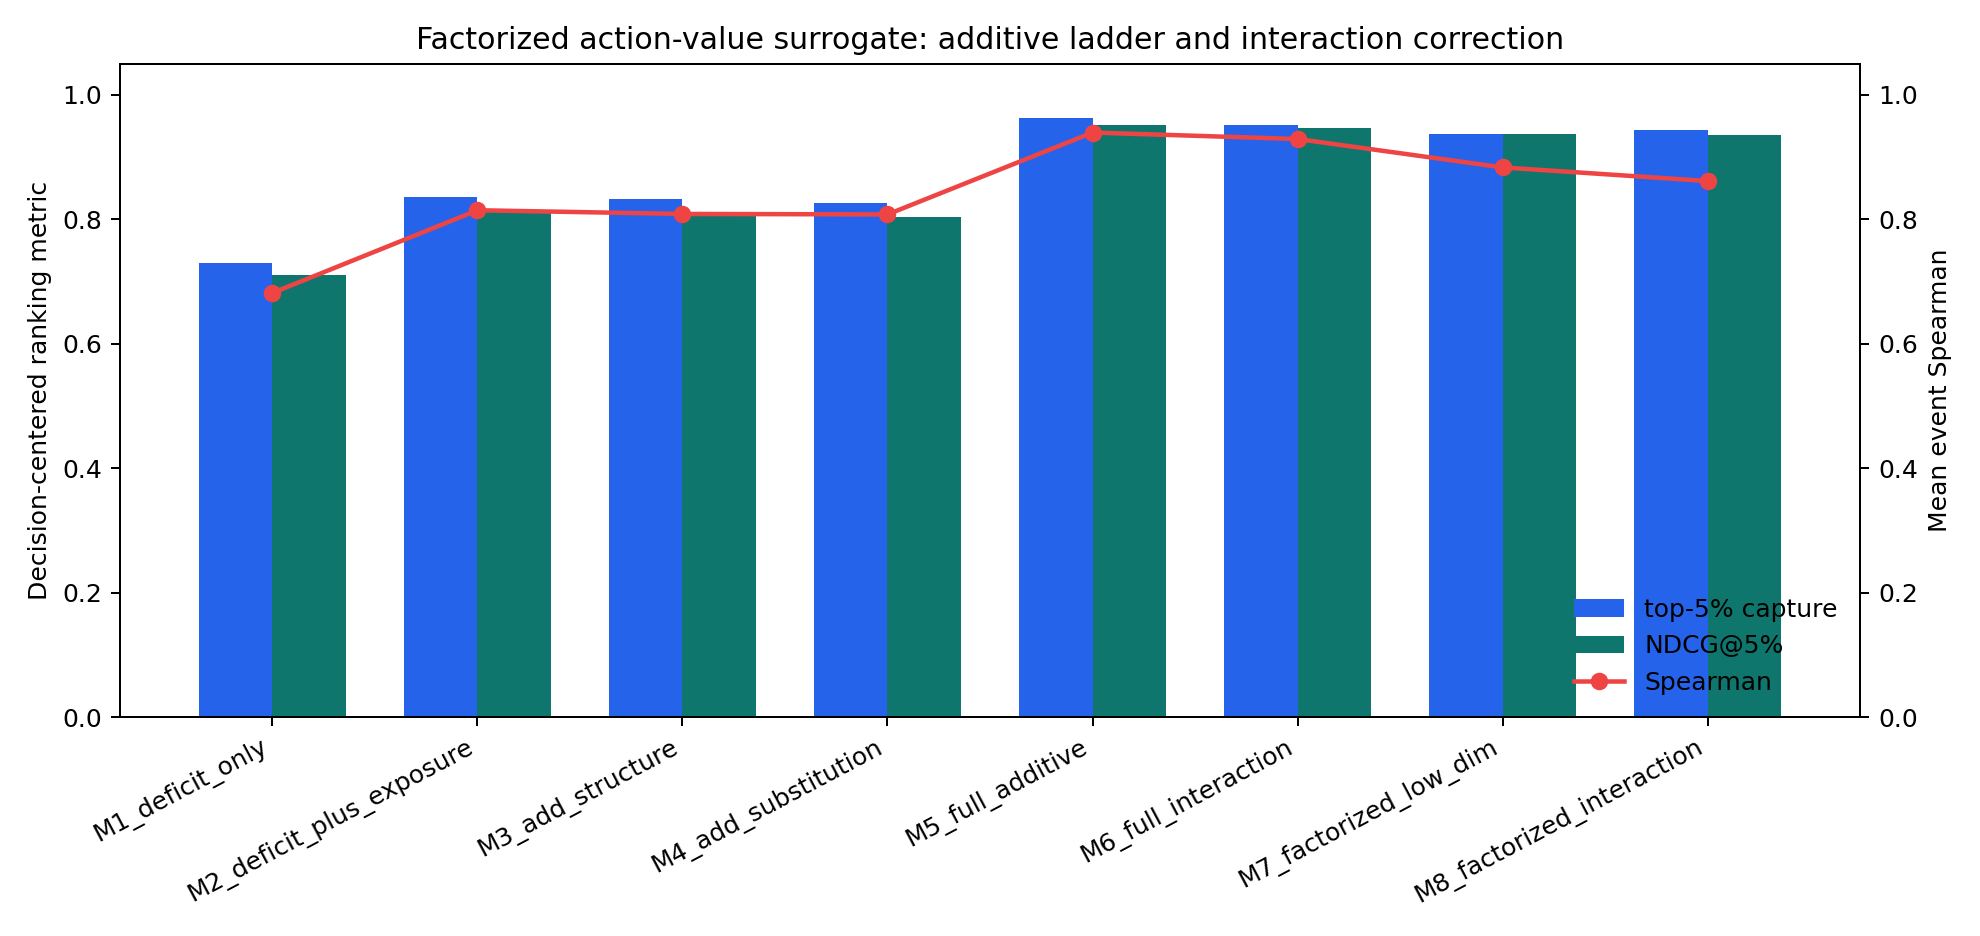
\includegraphics[width=0.88\linewidth]{../../results/factorized_action_surrogate/figures/factorized_model_ladder.png}
  \caption{Factorized action-value surrogate under leave-one-city-out validation. OD exposure and time-feasibility activation produce the largest decision-centered gains, while unrestricted interaction terms do not improve cross-city top-tail capture.}
  \label{fig:factorized-action-surrogate}
\end{figure}

The role of city structure is not merely a distributional artifact. To test this, we compare observed OD-dependency graph features with shuffled graph features that preserve each city's unit-level exposure and structural-feature distribution but break the alignment between a unit and its actual OD position. Under leave-one-city-out validation, a local dynamic model without OD graph information captures 0.6540 of oracle top-5 percent marginal value. Adding the observed OD graph raises this to 0.9624, whereas replacing the same graph variables with within-city shuffled counterparts gives only 0.6372. The observed-shuffled gap is positive in every city, with mean top-5 percent capture gain 0.3253. The same pattern remains in the seven-feature factorized law: observed OD alignment captures 0.9375, while shuffled OD alignment captures 0.7017. Thus the law is not simply ``recover high-deficit places'' or ``use cities with more concentrated exposure''; it depends on whether persistent loss, intervention timing, and the actual OD-exposure position of the action are spatially aligned.

We then ask whether this OD alignment result requires higher-order message passing over the OD graph. Deterministic one-hop and two-hop OD message summaries are informative by themselves: a local/action model augmented only with these messages captures 0.8835 of oracle top-5 percent marginal value. However, once scalar OD exposure, degree, and scarcity are already included, adding the message summaries increases top-5 percent capture only from 0.9624 to 0.9663. Adding the same messages to the seven-feature factorized law slightly lowers top-5 percent capture from 0.9375 to 0.9314, although it mildly improves mean event Spearman. This supports a parsimonious interpretation: actual OD spatial alignment is essential, but the current recoverability law does not require an opaque graph message-passing surrogate to explain the dominant top-tail value field.

\begin{figure}[t]
  \centering
  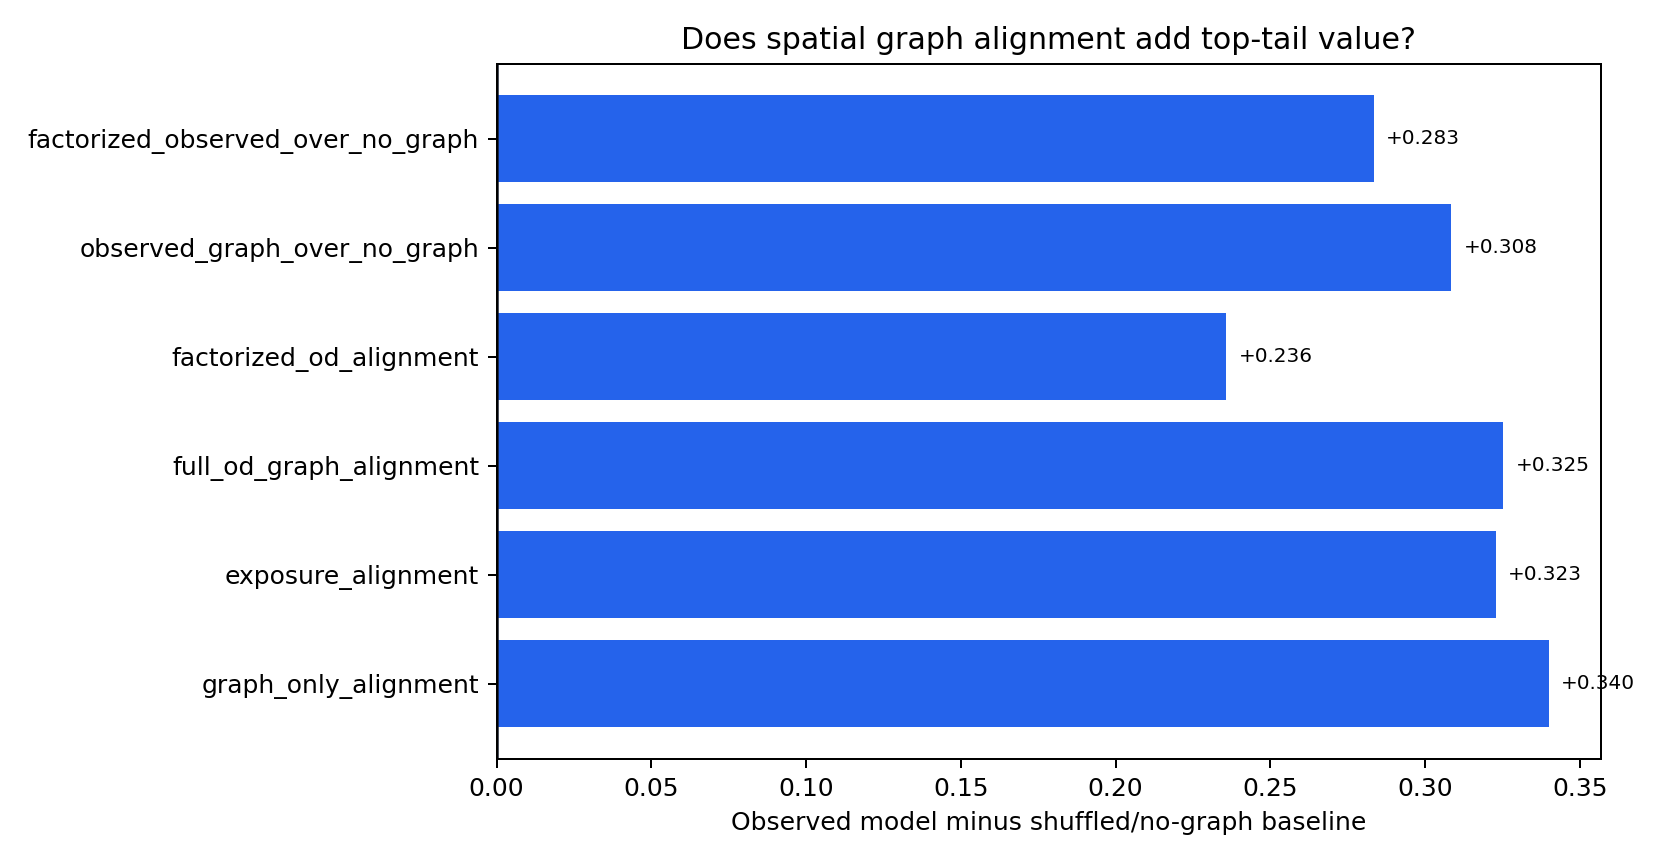
\includegraphics[width=0.86\linewidth]{../../results/graph_structure_ablation/figures/observed_vs_shuffled_graph_gaps.png}
  \caption{Observed OD graph alignment versus within-city shuffled graph features. Preserving graph-feature distributions while breaking unit alignment sharply reduces top-tail marginal-value capture, showing that OD spatial alignment is part of the recoverability law.}
  \label{fig:od-graph-alignment-ablation}
\end{figure}

We also test whether the law is regime-specific. Events are partitioned by total rainfall, peak rainfall, abnormal speed impact, rainfall duration, baseline loss, recoverable fraction, time of day, and weekday/weekend status. For each partition, an entire regime is held out and the surrogate is trained only on the remaining regimes. Across 24 held-out regimes, the seven-feature factorized law obtains mean top-5 percent value capture 0.9280; its weakest split is off-peak/night events, where capture remains 0.8880. The full additive surrogate reaches 0.9652, while adding explicit high-dimensional interaction terms lowers the mean to 0.9507. Thus the low-dimensional law is not merely memorizing a particular rainfall-intensity or time-of-day regime, although the full additive model still captures a small additional margin.

\begin{figure}[t]
  \centering
  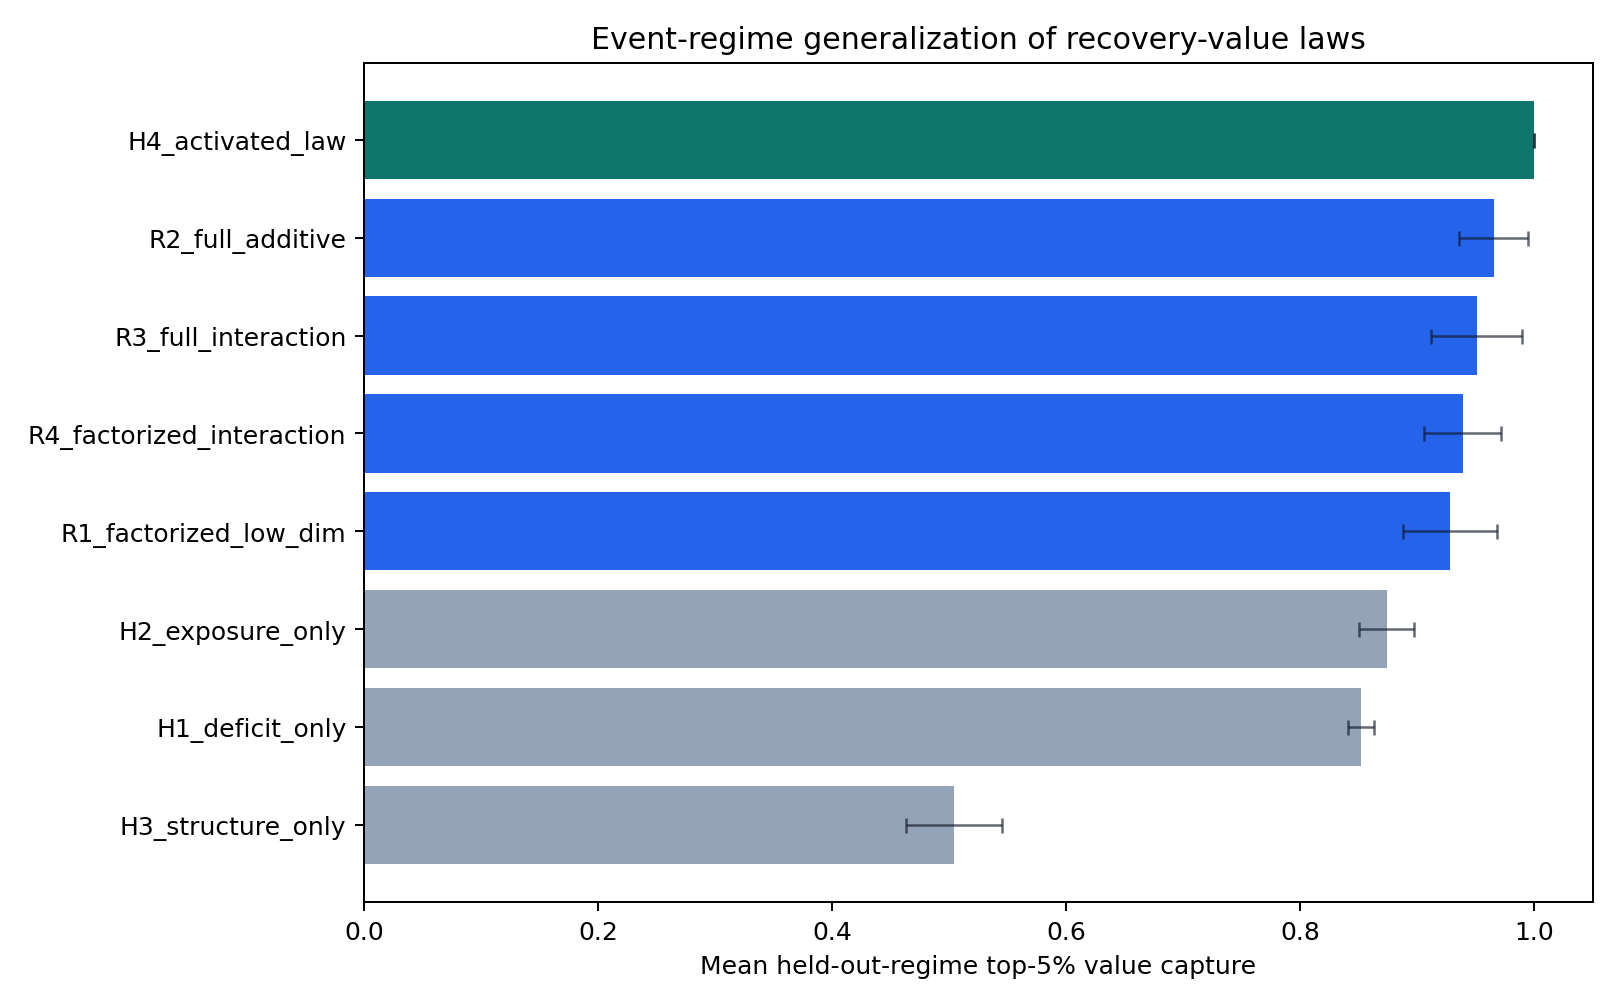
\includegraphics[width=0.86\linewidth]{../../results/event_regime_generalization/figures/regime_model_summary.png}
  \caption{Leave-event-regime-out validation. The compact factorized law remains close to the full additive surrogate when entire rainfall, speed-impact, duration, loss, and time-of-day regimes are held out.}
  \label{fig:event-regime-generalization}
\end{figure}

We further test chronological robustness. Because the current data cover one main speed month per city, calendar year is confounded with city composition: 2019 contains Chicago, Dallas, Houston, and New York; 2023 contains Philadelphia; and 2024 contains Austin and San Antonio. The main temporal test therefore holds out event-order periods within each city rather than treating year holdout as clean time extrapolation. Across five within-city early/middle/late and early/late chronological splits, the seven-feature factorized law obtains mean top-5 percent value capture 0.9248, with worst split 0.9074. The full additive surrogate reaches 0.9705, showing that richer context still carries additional information, but the compact law remains stable under same-city chronological holdout. A stricter forward audit that trains on earlier within-city events and tests on later events gives factorized mean capture 0.9148. Year holdout is reported only as a confounded audit, where factorized capture is 0.9592, because this split mixes temporal extrapolation with unseen city structure.

\begin{figure}[t]
  \centering
  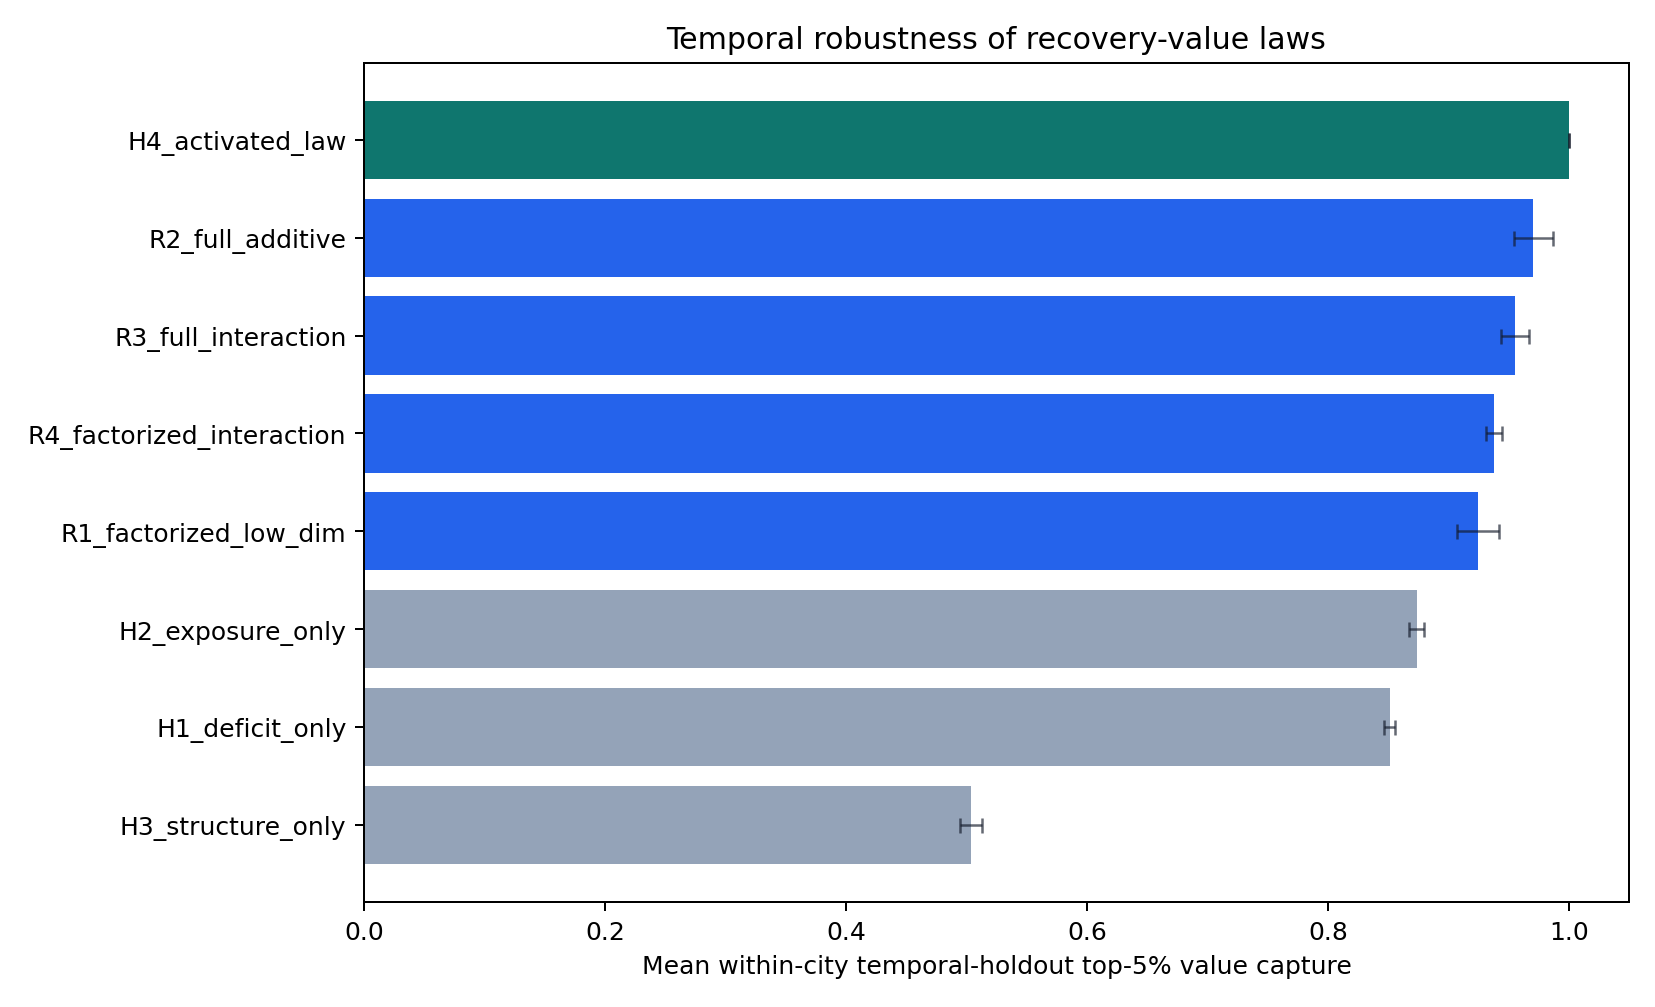
\includegraphics[width=0.86\linewidth]{../../results/temporal_generalization/figures/temporal_model_summary.png}
  \caption{Within-city chronological holdout validation. The compact factorized law remains stable when early, middle, late, or half-period event groups are held out within each city; calendar-year holdout is treated separately because it is city-confounded in the current sample.}
  \label{fig:temporal-generalization}
\end{figure}

As a final surrogate audit, we compare lightweight neural multilayer perceptrons with ridge models under strict and intentionally easier splits. Under leave-one-city-out validation, the full-feature MLP captures 0.9417 of oracle top-5 percent value, below the full ridge model's 0.9605. The seven-feature factorized MLP is essentially tied with factorized ridge, at 0.9329 versus 0.9346. A random-event split is easier for the full MLP, raising top-5 percent capture to 0.9573, while adding city identity to that split gives only a small gain of 0.0027. By contrast, adding event identity in a token-random split raises token-level Spearman correlation by 0.0162. This pattern is a useful guardrail: high-capacity nonlinear models and identity tokens can make token-level fit look excellent, but they do not replace strict city/event generalization or the compact structural law.

\begin{figure}[t]
  \centering
  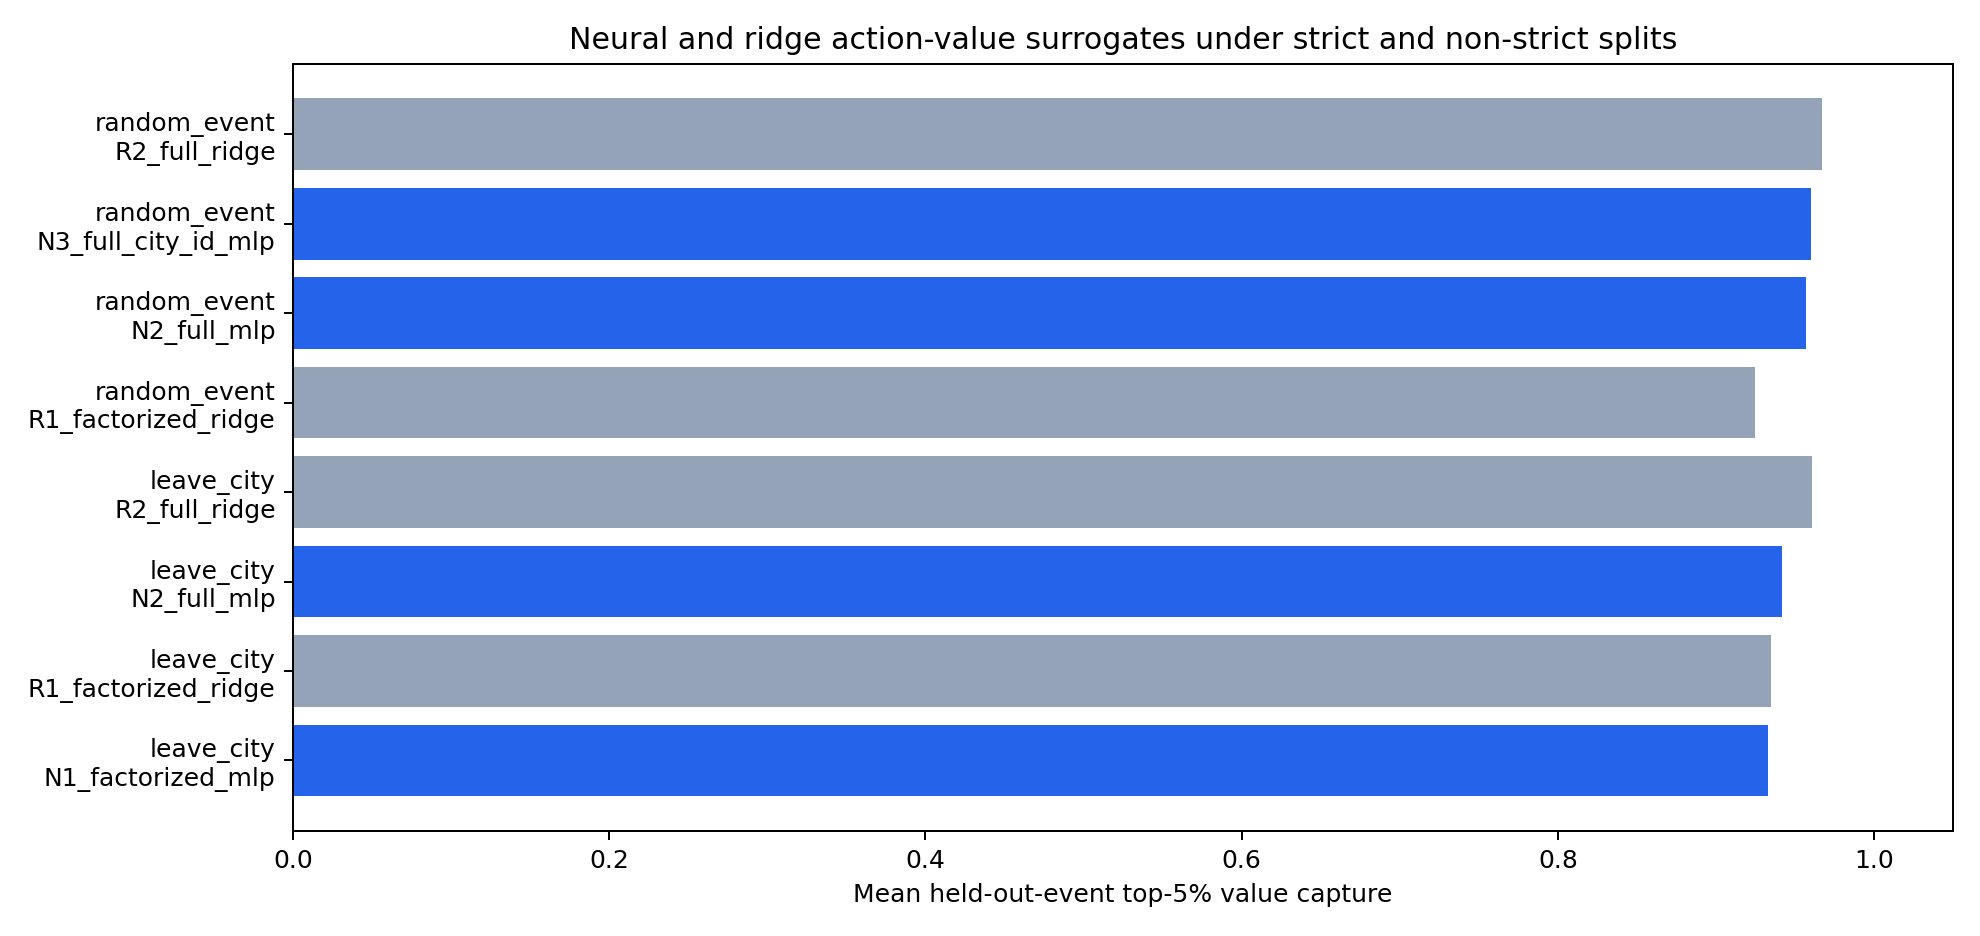
\includegraphics[width=0.86\linewidth]{../../results/neural_surrogate_leakage/figures/neural_split_model_summary.png}
  \caption{Neural surrogate and identity-leakage audit. Lightweight MLPs do not improve strict leave-city top-tail capture over ridge laws, while token-random identity features can inflate apparent fit.}
  \label{fig:neural-surrogate-leakage}
\end{figure}

Finally, we check whether these conclusions depend on a particular training objective. The main surrogate above uses ordinary log marginal-value regression, while the scientific evaluation is top-tail ranking. We therefore compare ordinary log-value regression with event-centered log regression, top-tail-weighted regression, rank-percentile regression, and event-standardized regression. For the seven-feature factorized law, ordinary log-value regression is already best: top-5 percent value capture is 0.9375, compared with 0.9323 for top-tail weighting and 0.8978 for rank-percentile regression. For the full additive surrogate, event-centered regression improves top-5 percent capture from 0.9624 to 0.9787. This supports using top-tail capture and regret as evaluation criteria, but it also shows that the compact law is not an artifact of a specialized ranking-loss trick.

We further separate city structure from intervention-parameter mechanics. A leave-one-city model that sees only the policy clock, response delay, intervention type, and budget captures 0.4997 of oracle top-5 percent value. Adding calibrated effectiveness per cost raises this to 0.5779, but adding OD exposure after local deficit features raises capture from 0.5899 to 0.8333. More directly, a parameter-light factorized law that omits \(\eta/c\) but keeps delay feasibility, future recoverable horizon, OD exposure, and intervention type already captures 0.9397, essentially matching the full factorized law with \(\eta/c\) at 0.9375. A fixed-channel diagnostic gives the same interpretation inside the first-order label field: within city-event-time-intervention groups, efficiency-only ranking captures 0.2012 of top-10 percent value, while the horizon--OD-exposure activation term nearly recovers the within-channel target. Thus the discovered law is conditional on the management regime, but it is not reducible to the regime parameters alone; spatial alignment between future loss and OD exposure remains the dominant source of top-tail action value.

We finally stress-test this boundary under parameter ensembles. Rather than re-solving the full LP for every management regime, this diagnostic recomputes the first-order action-value label under 11 eta, cost, delay, and channel-favored scenarios. A base-trained parameter-light factorized law, using delay feasibility, active future horizon, OD exposure, and intervention type but no absolute \(\eta/c\), obtains mean top-5 percent value capture 0.9095 across the perturbed scenarios, with a worst-scenario value of 0.7537. A base-trained factorized surrogate that includes absolute \(\eta/c\) is less stable under scale shifts, with mean capture 0.8774 and worst-scenario capture 0.7273 under the cheap-all scenario. The closed-form full activation score is exact in this diagnostic because the target is recomputed from the same first-order formula, so it should be read as a consistency check rather than independent causal validation. The result supports the structural part of the law---future recoverable horizon aligned with OD exposure and feasible channel timing---while motivating scenario augmentation before treating parameter-sensitive surrogates as robust across management regimes.

The formula-extraction stage makes this law explicit rather than leaving it as an informal interpretation. Candidate symbolic scores and leave-one-city log-linear formulas were evaluated on 170,137 action tokens from 105 city-events. The compact activated law lies on the accuracy--simplicity Pareto frontier; within the formula-extraction metric it has top-5 percent marginal-value capture 0.1121, compared with 0.0995 for the exposure-only symbolic term and 0.1026 for the minimal leave-city log-law. A feature-group ablation further shows that removing OD exposure and structural variables produces the largest top-tail capture drop, 0.0276. Thus the dominant empirical structure is not rainfall severity or budget alone, but the activation of future recoverable loss by OD exposure and feasible intervention efficiency.

The same action-token field also reveals why the law is not reducible to a one-factor heuristic. Ranking each city-event's candidate actions by highest remaining deficit captures 0.8520 of the oracle top-5 percent marginal value on average, but 24.3 percent of its top-ranked actions fall outside the true value top-20 percent. Exposure-only ranking is stronger, capturing 0.8706 of oracle top-tail value, but still has a 14.6 percent false-positive share. Structure-only ranking is the clearest counterexample: it captures only 0.5039 of oracle top-tail value, and 81.7 percent of its top-5 percent actions are outside the true value top-20 percent. Conversely, 34.2 percent of true top-5 percent actions do not appear in any simple top-5 percent ranking, and 83.9 percent of true top-5 percent actions are below the structure-only top-20 percent. The failure modes are also interpretable: deficit-only false positives commonly have below-median future horizon or low intervention efficiency, while structure-only false positives often lack the relevant OD exposure or efficient action channel.

\begin{figure}[t]
  \centering
  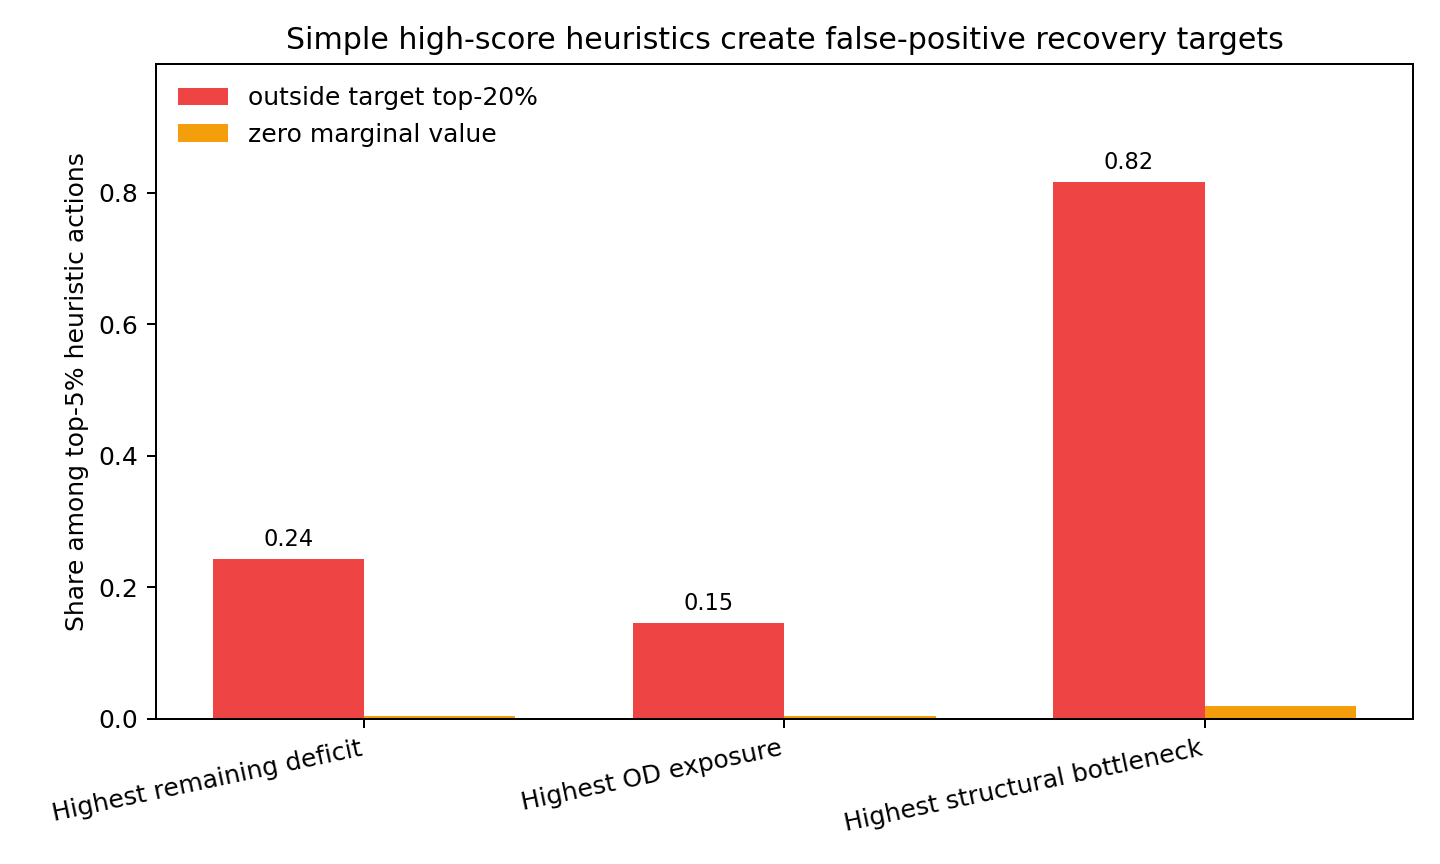
\includegraphics[width=0.84\linewidth]{../../results/nonobvious_action_laws/figures/heuristic_false_positive_rates.png}
  \caption{One-factor action heuristics create false recovery priorities. High deficit and high exposure are informative but incomplete; static structure alone is especially unreliable unless activated by persistent future loss, OD exposure, feasibility, and efficiency.}
  \label{fig:nonobvious-action-failures}
\end{figure}

The intervention mix of the true top-tail further clarifies the mechanism. Among target top-5 percent action tokens, temporary capacity \(C\) accounts for 66.5 percent of actions and 77.1 percent of top-tail value, substitution/control \(S\) accounts for 15.7 percent of actions and 17.1 percent of value, and durable restoration \(R\) accounts for 17.8 percent of actions but only 5.8 percent of value in the first-order field. This does not mean \(R\) is unimportant in the finite-budget LP; rather, it shows that short-window marginal value is strongly shaped by response delay, immediate feasibility, and the channel through which loss propagates.

The current data do not yet cleanly separate peak disturbance from cumulative disturbance at the region level, because the observed event signal is projected spatially through the same destination-vulnerability profile. Therefore the peak-versus-persistence result should be framed cautiously: the robust finding is not that the peak term is irrelevant, but that action value depends on future remaining reducible loss after accounting for OD exposure, timing, and resource efficiency.

\begin{figure}[t]
  \centering
  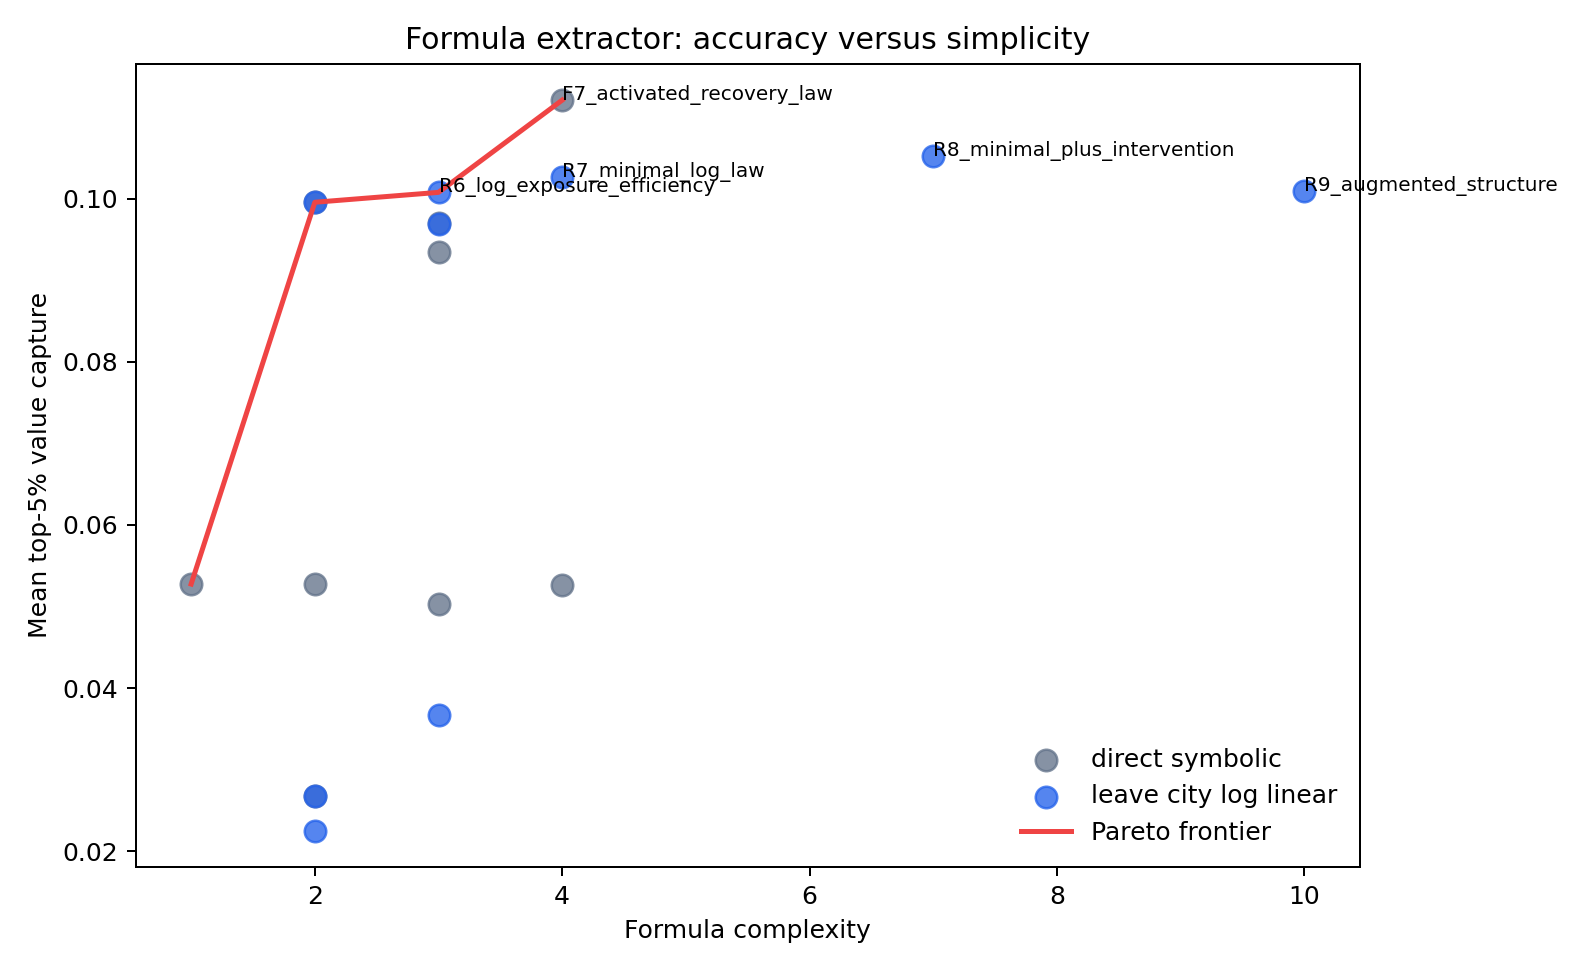
\includegraphics[width=0.82\linewidth]{../../results/symbolic_law_extraction/figures/formula_complexity_capture.png}
  \caption{Symbolic formula extraction compares compact hand-readable laws with leave-city log-linear extractors. The activated law remains on the accuracy--simplicity Pareto frontier.}
  \label{fig:symbolic-formula-extraction}
\end{figure}

\subsection{Finite-Budget Residual Law}

The first-order action law is not sufficient for the complete resource-allocation problem. Static small-signal greedy allocation captures 0.8228 of base LP recovery gain on average, leaving a finite-budget gap. The gap is explained by local saturation, diminishing returns, overlapping effects on the same loss channel, period-budget constraints, and substitution among the three intervention primitives. In the finite-budget analysis, the LP uses about 1.67 times as many distinct actions as static greedy and has a mean action-cost Jaccard overlap of 0.6127 with it, showing that the optimizer spreads resources more broadly to avoid exhausting high first-order locations.

The corrected finite-budget law is therefore residual rather than static. After each deployment pass, the current residual states \(b\), \(r^C\), \(r^S\), and \(\ell\) are replayed; candidate segments are then re-scored against the remaining loss:
\begin{equation}
v_{s \mid x}^{\mathrm{res}}
  \propto
  \frac{1}{L_0\,C_s}
  \sum_{\tau>t_s}
    W_{s,\tau}
    \min\{
      \Delta_s \rho_{s,\tau},
      R_{s,\tau}(x)
    \},
\end{equation}
where \(s\) is a deployment segment, \(x\) is the current residual state, \(C_s\) is segment cost, \(\Delta_s\rho_{s,\tau}\) is the decayed segment effect at future time \(\tau\), and \(R_{s,\tau}(x)\) is the remaining reducible loss in the relevant channel. This is still an interpretable law rather than a new LP solve: it updates the state, applies a finite-loss truncation, and greedily allocates the next budget batch.

This residual law nearly closes the base-scenario LP gap. Across 105 city-events, residual finite greedy captures 0.9736 of the base LP gain on average, with median 0.9921, compared with 0.8228 for static small-signal greedy. The mean improvement over static greedy is 0.1508 of LP gain, and positive improvement appears in 91.4 percent of events. The gains are largest in cities where static greedy suffered from stronger saturation and interaction effects, including Chicago, Philadelphia, and San Antonio; Dallas is already nearly solved by the static ranking, so residual replanning adds little.

\subsection{Robustness Across Budget and Delay}

The residual law remains stronger than static ranking under budget and response perturbations. In the 105-event stress test, residual replanning captures 0.5711 of base LP gain under low budget, 0.9660 in the base scenario with coarser ten-pass replanning, 1.5916 under high budget measured against the base LP denominator, 0.8780 with two additional hours of delay, 0.7734 with four additional hours of delay, and 0.5222 under scarce-and-late conditions. These stress-test numbers are normalized by the base LP gain, so they show policy stability rather than scenario-specific optimality.

A separate fine-grained budget-leverage sweep tests whether decision leverage is highest at an intermediate resource level. Using ten budget scales from 0.10 to 3.00, this specific interior-peak hypothesis is not supported in the current action-value proxy and LP replay setting. The absolute law-versus-random replay advantage rises from 0.0026 at budget scale 0.10 to 0.0144 at 1.00 and 0.0278 at 3.00, and every city has its largest absolute replay advantage at the largest tested budget. However, leverage per unit budget falls from 0.0259 at 0.10 to 0.0144 at 1.00 and 0.0093 at 3.00, while the law/random replay-gain ratio falls from 10.02 to 5.56 and then 3.90. Thus the better budget law in this sample is scale-dependent diminishing leverage: larger budgets increase the total amount of recoverable value captured, but each additional unit of budget carries less incremental decision advantage.

We then re-solve budget-specific full LP optima for one representative event per city over the same ten budget scales. All 70 representative LP closures solve to optimality. This stronger closure gives the same budget shape: mean LP recoverable fraction rises from 0.0219 at budget scale 0.10 to 0.1342 at 1.00 and 0.2904 at 3.00, but LP gain per unit budget falls from 0.0312 to 0.0201 and then 0.0148. The activated law captures 0.7829 of the budget-specific LP gain at the base budget and 0.8004 on average over all representative budget rows, while random-positive captures only 0.1488 at the base budget. The law-random advantage normalized by the budget-specific LP gain is strongest at the lowest budget, falling from 0.7784 at 0.10 to 0.6341 at 1.00 and 0.5733 at 3.00. Thus the diminishing-leverage result is not only a proxy denominator artifact.

\begin{figure}[t]
  \centering
  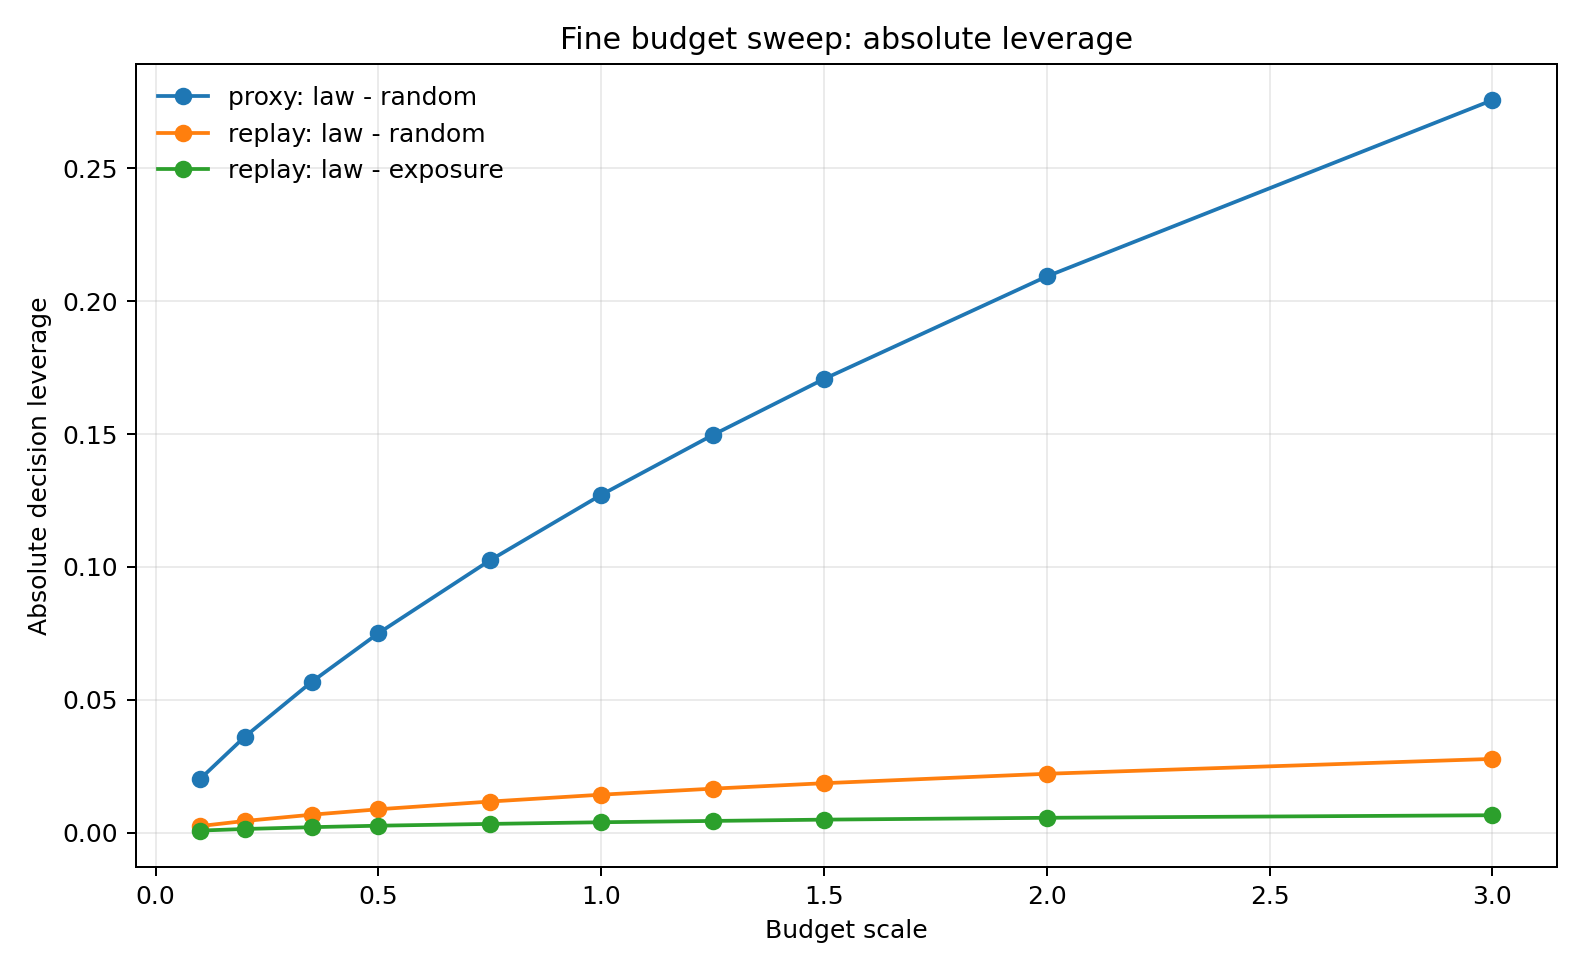
\includegraphics[width=0.84\linewidth]{../../results/budget_fine_sweep/figures/fine_budget_leverage_curve.png}
  \caption{Fine budget-leverage sweep. Absolute law-guided advantage grows across the tested budget range, while separate relative and per-budget diagnostics show diminishing decision leverage.}
  \label{fig:budget-leverage-phase}
\end{figure}

To test scenario-specific closure directly, representative non-base LP optima were re-solved for selected city-events. Among 23 successful non-base LP closures, static small-signal greedy captures 0.7228 of the scenario LP gain on average, while residual finite greedy captures 0.9411. The residual policy weakly dominates or ties static greedy in all successful closures. Five hard non-base cases reached the current time limit, so this result should be read as representative scenario-optimum validation rather than full non-base closure over all 105 events.

We also re-solve full LP optima under intervention-parameter ensembles. For four representative city-events and five eta, cost, delay, or channel-favored scenarios, all 20 parameter-scenario LPs solve to optimality. Static small-signal greedy captures 0.7451 of each scenario's LP gain on average, whereas residual finite greedy captures 0.9662, with positive improvement in every tested event-scenario. The weakest residual scenario is \(R\)-favored restoration, where residual finite greedy still captures 0.9516 of the scenario-specific LP gain. This extends the first-order parameter-ensemble result: the structural action-value law becomes most reliable as a finite-budget policy when it is repeatedly re-scored against the residual state.

We also test whether action importance is stable to near-neighbor optimization problems. For four representative interaction-sensitive events, intervention effectiveness and cost are perturbed three times within a clipped 20 percent range and the LP is re-solved. The original base LP action set captures 0.7954 of the perturbed LP selection-frequency mass, residual finite greedy captures 0.6097, and static small-signal greedy captures 0.4659. Thus residual replanning is closer than static ranking to the perturbed stable action core, but the exact action list remains parameter-sensitive. This supports using the learned result as a value law rather than as a fixed list of universal intervention locations.

\begin{figure}[t]
  \centering
  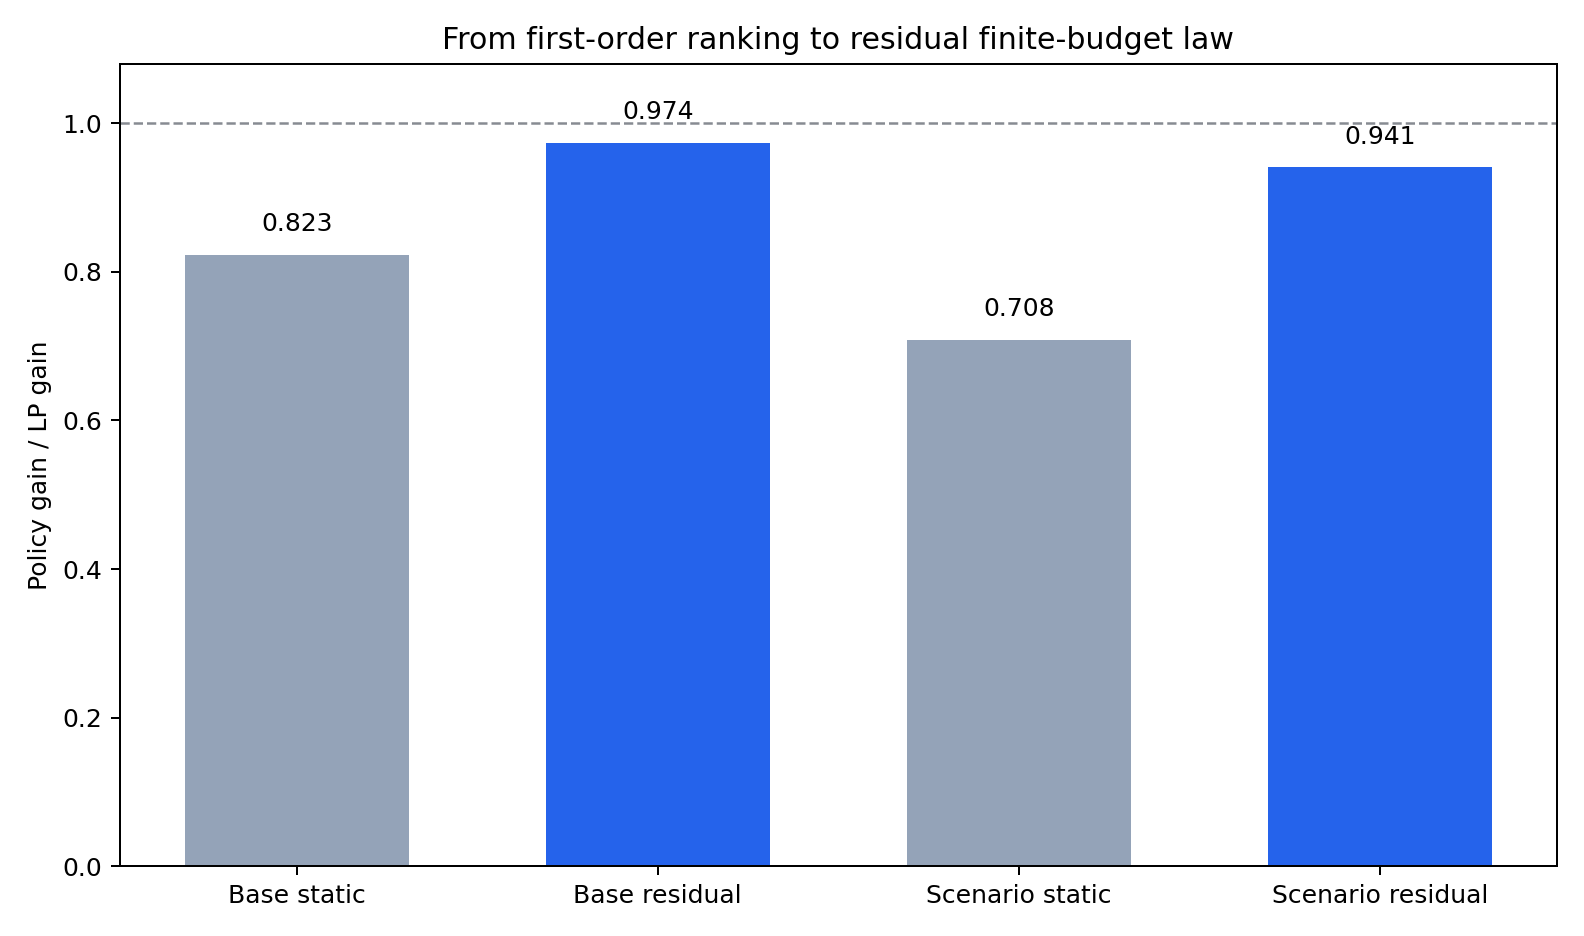
\includegraphics[width=0.85\linewidth]{../../results/law_synthesis/figures/law_evidence_ladder.png}
  \caption{Policy gain captured by static and residual laws under base and representative non-base LP closures. Residual replanning turns the first-order marginal law into a finite-budget allocation law.}
  \label{fig:law-evidence-ladder}
\end{figure}

\subsection{Event-Level Top-Tail Law}

The action-value field also defines an event-level law. A rainfall event is decision-critical when recoverable value is concentrated in a small top tail of candidate actions. Across the 105 base events, the mean top-5 percent marginal-value share is 0.1645 and the mean marginal-value Gini is 0.4494. Decision-criticality is strongly associated with top-tail inequality: the Spearman correlation between marginal-value Gini and decision-criticality score is 0.8412, and the correlation between top-5 percent value share and decision-criticality is 0.7650. By contrast, baseline loss magnitude has negative Spearman correlation with decision-criticality in this sample. Thus large disruptions are not automatically the most decision-critical; moderate events can have high decision leverage when recoverable value is concentrated on a small set of exposed, intervention-sensitive locations.

A severity-decoupling audit makes this contrast concrete. Using rank thresholds, there are 13 high-loss but low-decision-critical events and 19 moderate-or-lower-loss but high-decision-critical events; 16 high-rain events also fall below the decision-criticality median. In leave-city event-level prediction, severity-only features have near-zero pooled Spearman correlation with decision-criticality (-0.0402), whereas top-tail structure features reach 0.6790. This event-level law is therefore not a rainfall-severity law. Its current boundary is equally important: the top-5 percent value share has a between-city variance share of 0.5990, so the present event-level signal is partly a city-structure signal induced by OD exposure and current spatial calibration. A finer zone-level rainfall and speed footprint would be needed before claiming that within-city event footprint variation is fully resolved.

\begin{figure}[t]
  \centering
  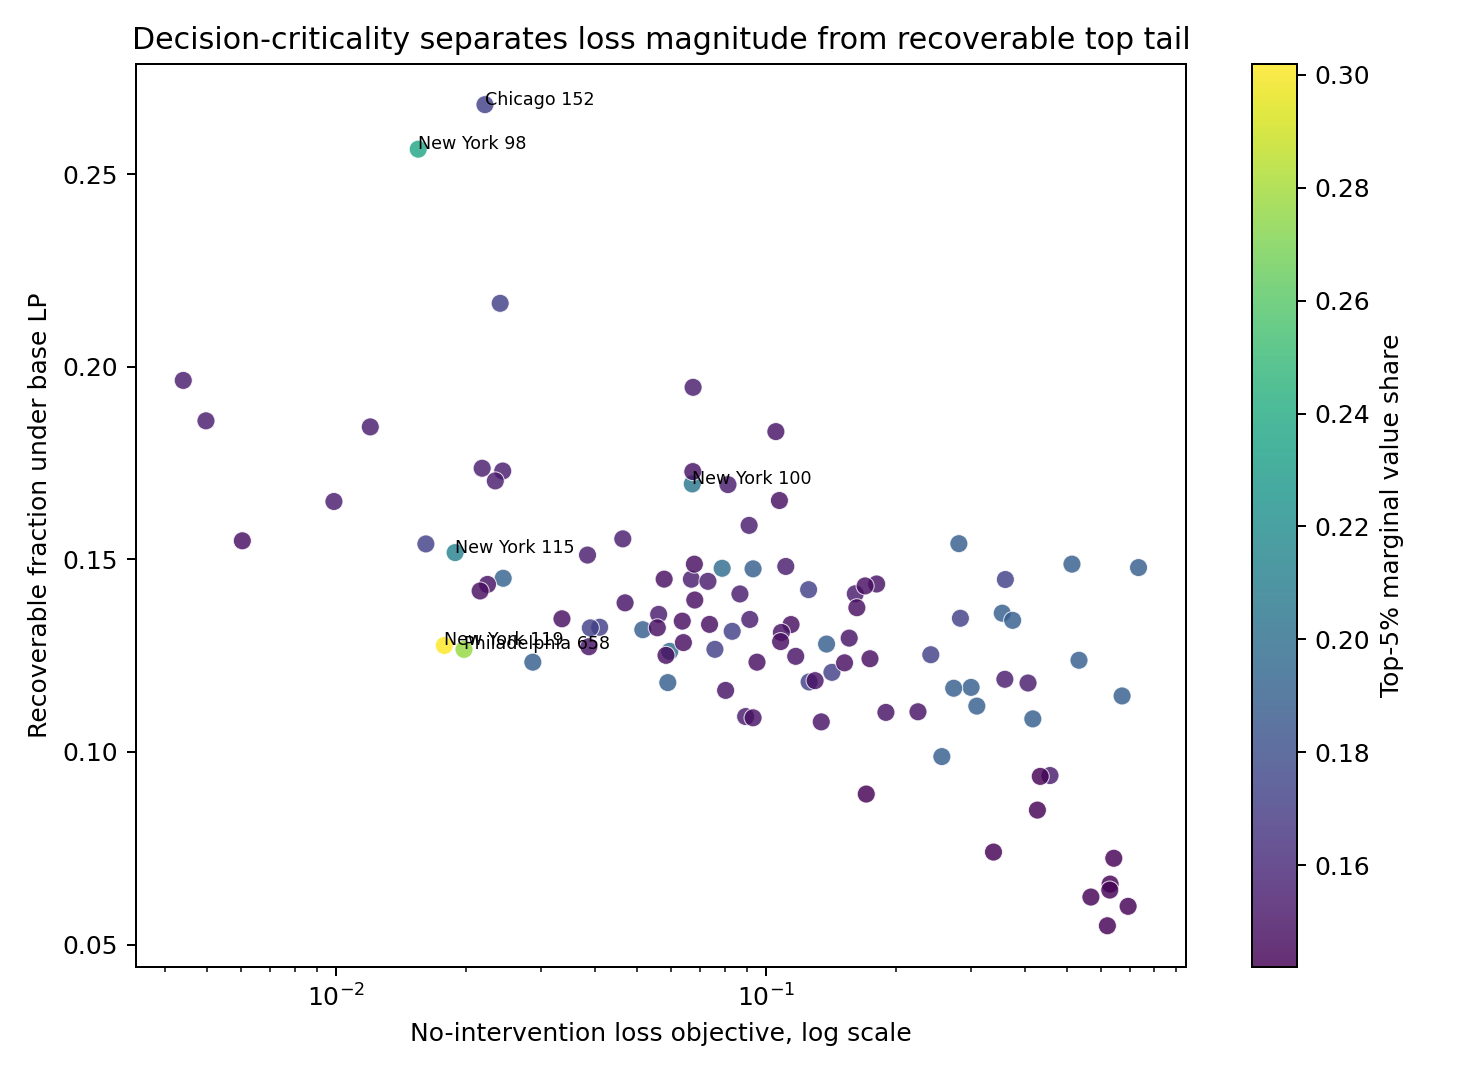
\includegraphics[width=0.85\linewidth]{../../results/law_synthesis/figures/event_top_tail_phase.png}
  \caption{Event-level recoverability and top-tail concentration. The highest decision-critical events are not simply the largest loss events; they combine recoverable fraction with a concentrated marginal-value top tail.}
  \label{fig:event-top-tail-law}
\end{figure}

Together, the action-level and event-level findings support the paper's central claim: managed recoverability is not determined by disruption magnitude alone. It emerges when persistent functional loss, OD exposure, intervention feasibility, and finite-budget residual interactions align, and intelligent management matters most when this recoverable value forms a heavy top tail.

\subsection{Hindsight Boundary and Early Signals}

The main analysis should be interpreted as hindsight counterfactual recoverability: it uses the observed 12-hour disruption trajectory to ask how much loss was theoretically recoverable under a standardized management regime. A supplementary early-window test examines whether decision-critical events can be detected before the full trajectory is known. Using leave-one-city-out ridge models on aggregate information from the first 1, 2, 3, 6, or 12 hours, the best early model for decision-criticality uses first-hour speed-abnormality plus static city-structure features and obtains Spearman correlation 0.8353. With the first two hours and all early features, decision-criticality Spearman is 0.7964 and top-20 percent recall is 0.6190. Recoverable fraction is harder to identify early: the two-hour all-feature Spearman is 0.5990, while the best value appears only when the full 12-hour window is available.

The decomposition is important. At the one-hour window, static city features alone have Spearman 0.7675 with final decision-criticality, early speed features have 0.5272, and rainfall-only features have negative correlation in this sample. Thus early predictability is not simply a rainfall-nowcasting result. It arises because some cities and early abnormal-speed states already reveal whether recoverable value is likely to concentrate in a top tail. This supports limited early warning of decision-criticality, but it does not convert the study into a fully online control model.

\begin{figure}[t]
  \centering
  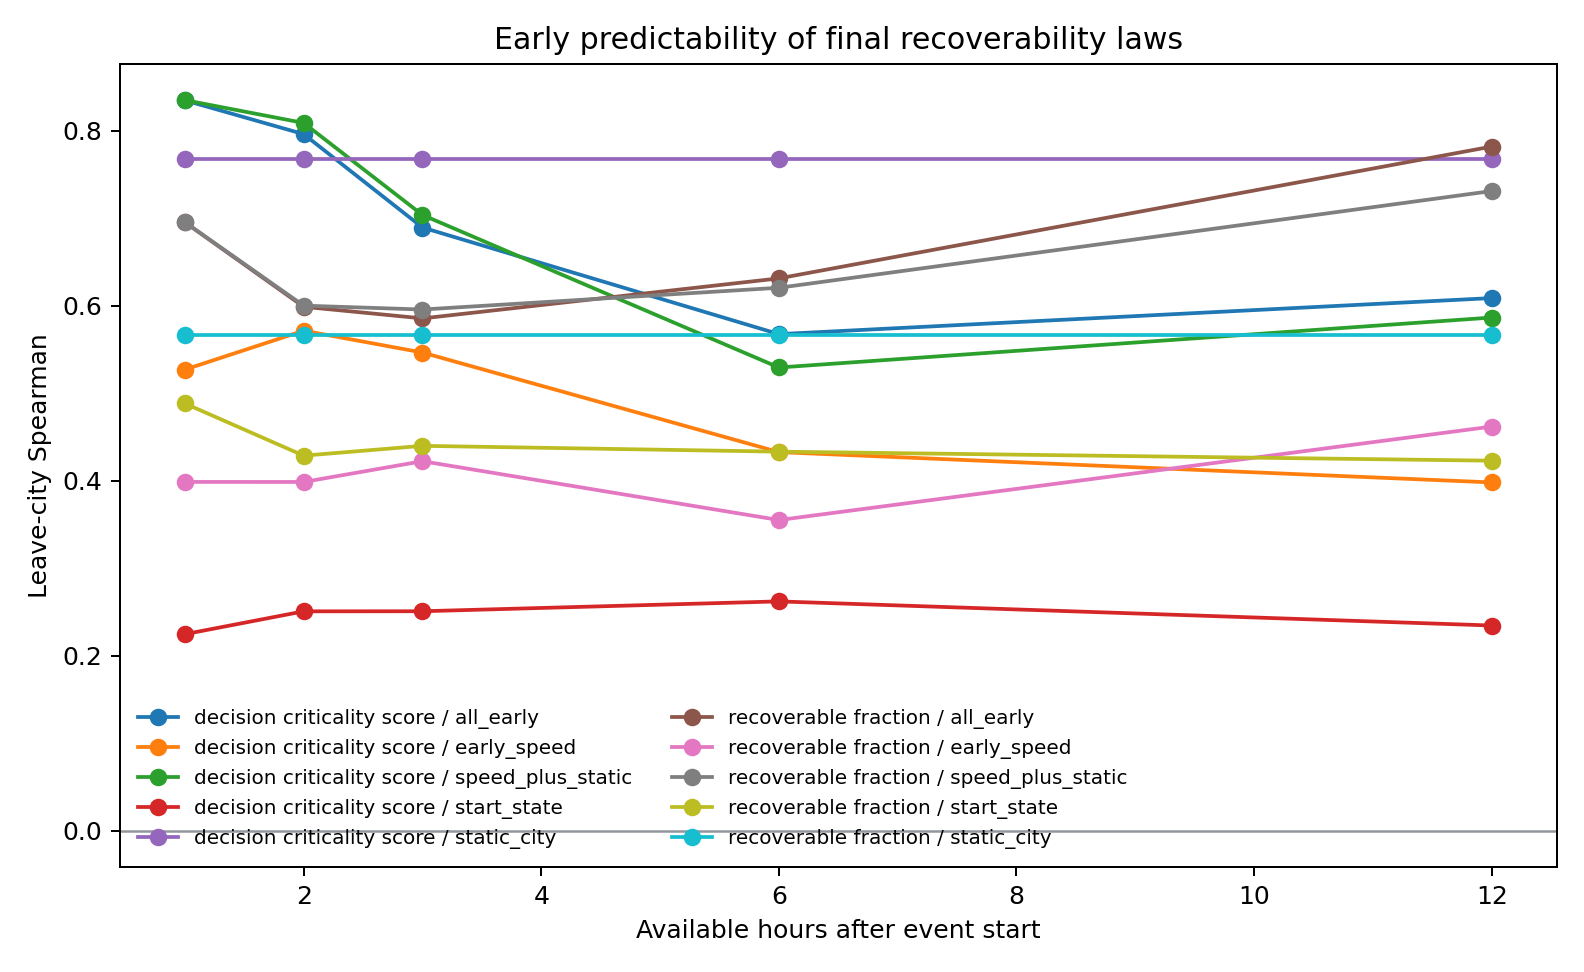
\includegraphics[width=0.84\linewidth]{../../results/early_predictability/figures/early_predictability_spearman.png}
  \caption{Early-window predictability of final recoverability quantities under leave-one-city-out validation. Decision-criticality is partly identifiable from early speed and static structure, while recoverable fraction depends more strongly on the full trajectory.}
  \label{fig:early-predictability}
\end{figure}
